\chapter{通过真核生物 RNA-Seq 数据估计基因的转录组问题为 NP 难}
\label{chap-rna-seq-nphard}

\section{问题描述}
在真核生物 RNA-Seq 数据处理过程当中, 重要的一步是通过 RNA-Seq 数据估计出基因的转录组. 
由于在真核生物的转录过程当中会有选择性剪切的现象发生, 一个基因可能转录出多个剪切异构体. 
在这种情况下, 我们需要通过 RNA-Seq 数据估计出转录本的组成. 
在这里我们首先对通过真核生物 RNA-Seq 数据估计基因的转录组的问题, 
亦即对基因的剪切异构体的辨识, 进行描述. 

在 RNA-Seq 实验中得到的读段数据在比对到参考基因组序列上如图 \ref{nphard.ex1.aligned.data} 所示. 
对于 RNA-Seq 数据, 
我们可以通过序列拼装工具 (例如 Trinity \cite{grabherr2011full} 等) 进行拼装. 
得到每一个基因的外显子的序列以及这些外显子之间是如何连接在一起的关系, 
从而得到每一个基因的剪切图 \cite{Heber01072002}. 
在有基因的参考序列以及基因注释的情况下, 也可以直接通过基因注释获得每一个基因的剪切图. 
对于图 \ref{nphard.ex1.aligned.data} 中所示的基因和 RNA-Seq 数据, 
通过 Trinity 拼装获得的剪切图如图 \ref{nphard.ex1.splicing.graph} 所示. 

\begin{figure}[!t]
\centering
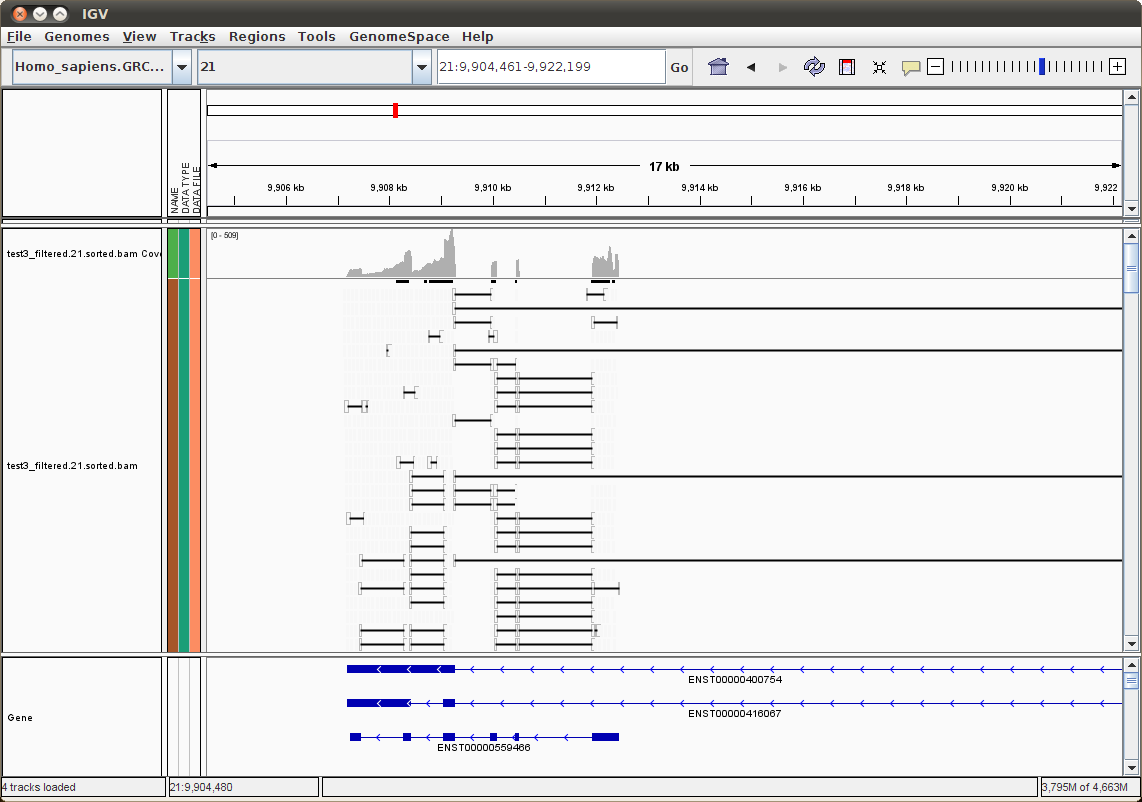
\includegraphics[width=\textwidth]{figures/nphard/comp1.png}
\caption{一个基因的比对到基因组参考序列上的 RNA-Seq 数据}
\label{nphard.ex1.aligned.data}
\end{figure}

\begin{figure}[!t]
\centering
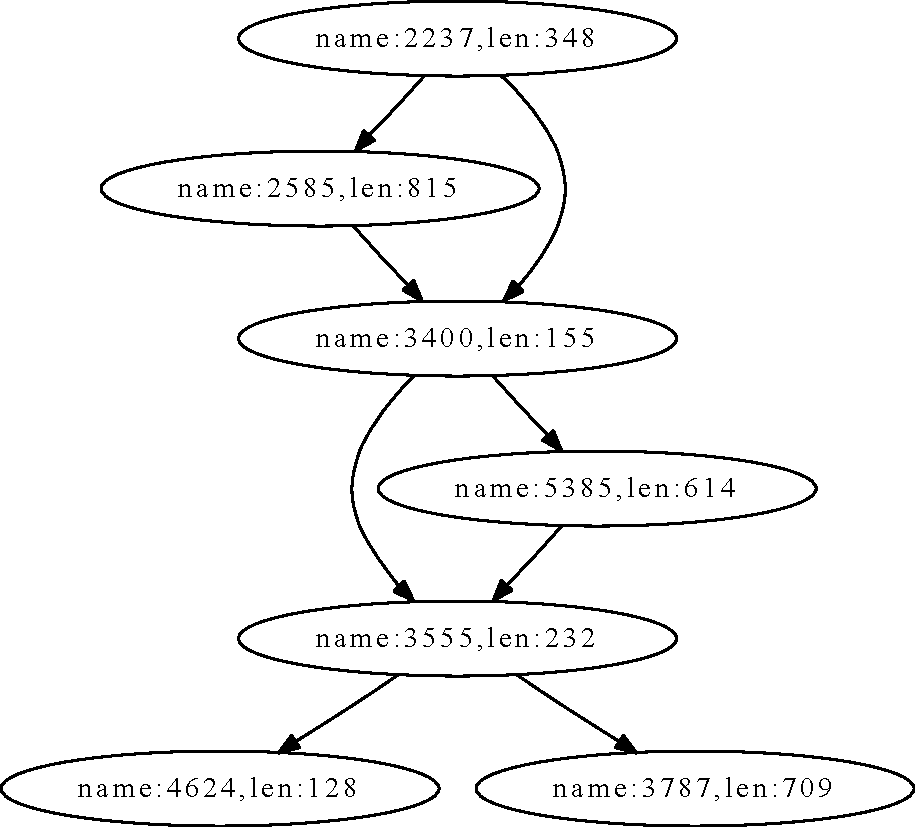
\includegraphics[width=\textwidth]{figures/nphard/comp1.pdf}
\caption{图 \ref{nphard.ex1.aligned.data} 中所示的基因和 
RNA-Seq 数据通过 Trinity 拼装得到的剪切图}
\label{nphard.ex1.splicing.graph}
\end{figure}

\subsection{模型}

为了能够通过 RNA-Seq 数据估计出转录组中转录本的组成, 辨识每个基因的剪切异构体, 
我们在这里介绍一个 Poisson 模型用来描述 RNA-Seq 数据 \cite{Jiang15042009}. 
该模型与 \ref{rna-seq-general-model} 中所介绍的多项式模型在数学上是等价的 
\cite{2011arXiv1104.3889P}. 
在这里采用 RNA-Seq 数据的 Poisson 模型是为了简化问题的描述. 

另外, 为了叙述的方便, 我们在这里纸考虑辨识一个基因的剪切异构体. 

对于真核生物中的一个基因, 根据剪切图的定义, 
我们将其表示为一个有向无环图 $G=(V,E)$, 其中 $G$ 中的一个节点代表一个外显子, 
节点 $v_i$ 到 $v_j$ 有一条边当且仅当在这个基因当中有一个剪切异构体同时包含 
$v_i$ 和 $v_j$ 所代表的外显子, 
同时在这个剪切异构体中 $v_i$ 和 $v_j$ 所代表的外显子是相邻的, 
并且 $v_i$ 代表的外显子在 $v_j$ 代表的外显子的 5' 上端. 

\subsection{M-ISOFORM 判定问题}

\section{证明}

